\documentclass[aspectratio=169,xcolor=table]{beamer}
\usepackage[utf8]{inputenc}
\usepackage[T1]{fontenc}
\usepackage{lmodern}
\usepackage[portuguese]{babel}
\usepackage{tabularx,booktabs}
\usetheme{DCC}
\setbeamertemplate{itemize items}[circle]
\setlength{\parskip}{0.5em}
\setbeamersize{text margin left=1cm,text margin right=0.6cm}
\graphicspath{{imgs/}}
\author[João Victor, Lucas Rapozo, Antoniel Magalhães]{\textbf{João Victor}\\[0.12cm]\textbf{Lucas Rapozo}\\[0.12cm]\textbf{Antoniel Magalhães}}
\title{From Tokens to Words:\\On the Inner Lexicon of LLMs}
\date{}
\newcommand{\fonte}[1]{\par\vspace{0.12cm}{\scriptsize\color{gray}Fonte: Kaplan et al. (ICLR 2025), #1.}}
\begin{document}
\hypersetup{pdfauthor={João Victor, Lucas Rapozo, Antoniel Magalhães},pdftitle={From Tokens to Words: On the Inner Lexicon of LLMs}}
% 1 | 0:00--0:20 | João Victor
\begin{frame}[plain,noframenumbering]\titlepage\end{frame}
% 2 | 0:20--1:15 | João Victor
\begin{frame}{O problema: palavras chegam fragmentadas}
\begin{block}{Exemplo de divisão artificial usado no artigo}
\centering\Large \texttt{cats} $\longrightarrow$ \texttt{ca} + \texttt{ts}
\end{block}
\begin{itemize}\setlength{\itemsep}{0.65em}
\item O tokenizador converte o texto em unidades que podem ser menores que uma palavra.
\item Uma palavra fora do vocabulário de tokens únicos ainda pode ser representada por vários tokens.
\item \textbf{Pergunta:} o modelo reconstrói internamente a palavra inteira? Onde e como isso acontece?
\end{itemize}
\fonte{seções 1 e 4.1}
\end{frame}
% 3 | 1:15--2:20 | João Victor
\begin{frame}{Hipótese: um léxico além do tokenizador}
\begin{itemize}\setlength{\itemsep}{0.65em}
\item \textbf{Vocabulário do tokenizador:} unidades com identificadores e vetores de entrada próprios.
\item \textbf{Léxico interno:} representações de palavras que emergem nos cálculos do modelo, inclusive palavras de vários tokens.
\item \textbf{Local proposto:} o estado interno do último token concentra informação sobre a palavra completa.
\item O estudo investiga Llama2-7B, Llama3-8B, Mistral-7B e Yi-6B; os resultados destacados a seguir são do Llama2-7B.
\end{itemize}
\fonte{seções 2--4; léxico distribuído, não um dicionário literal}
\end{frame}
% 4 | 2:20--3:20 | João Victor
\begin{frame}{Mecanismo proposto: agregar e reconstruir}
\begin{columns}[c,onlytextwidth]
\begin{column}{0.55\textwidth}
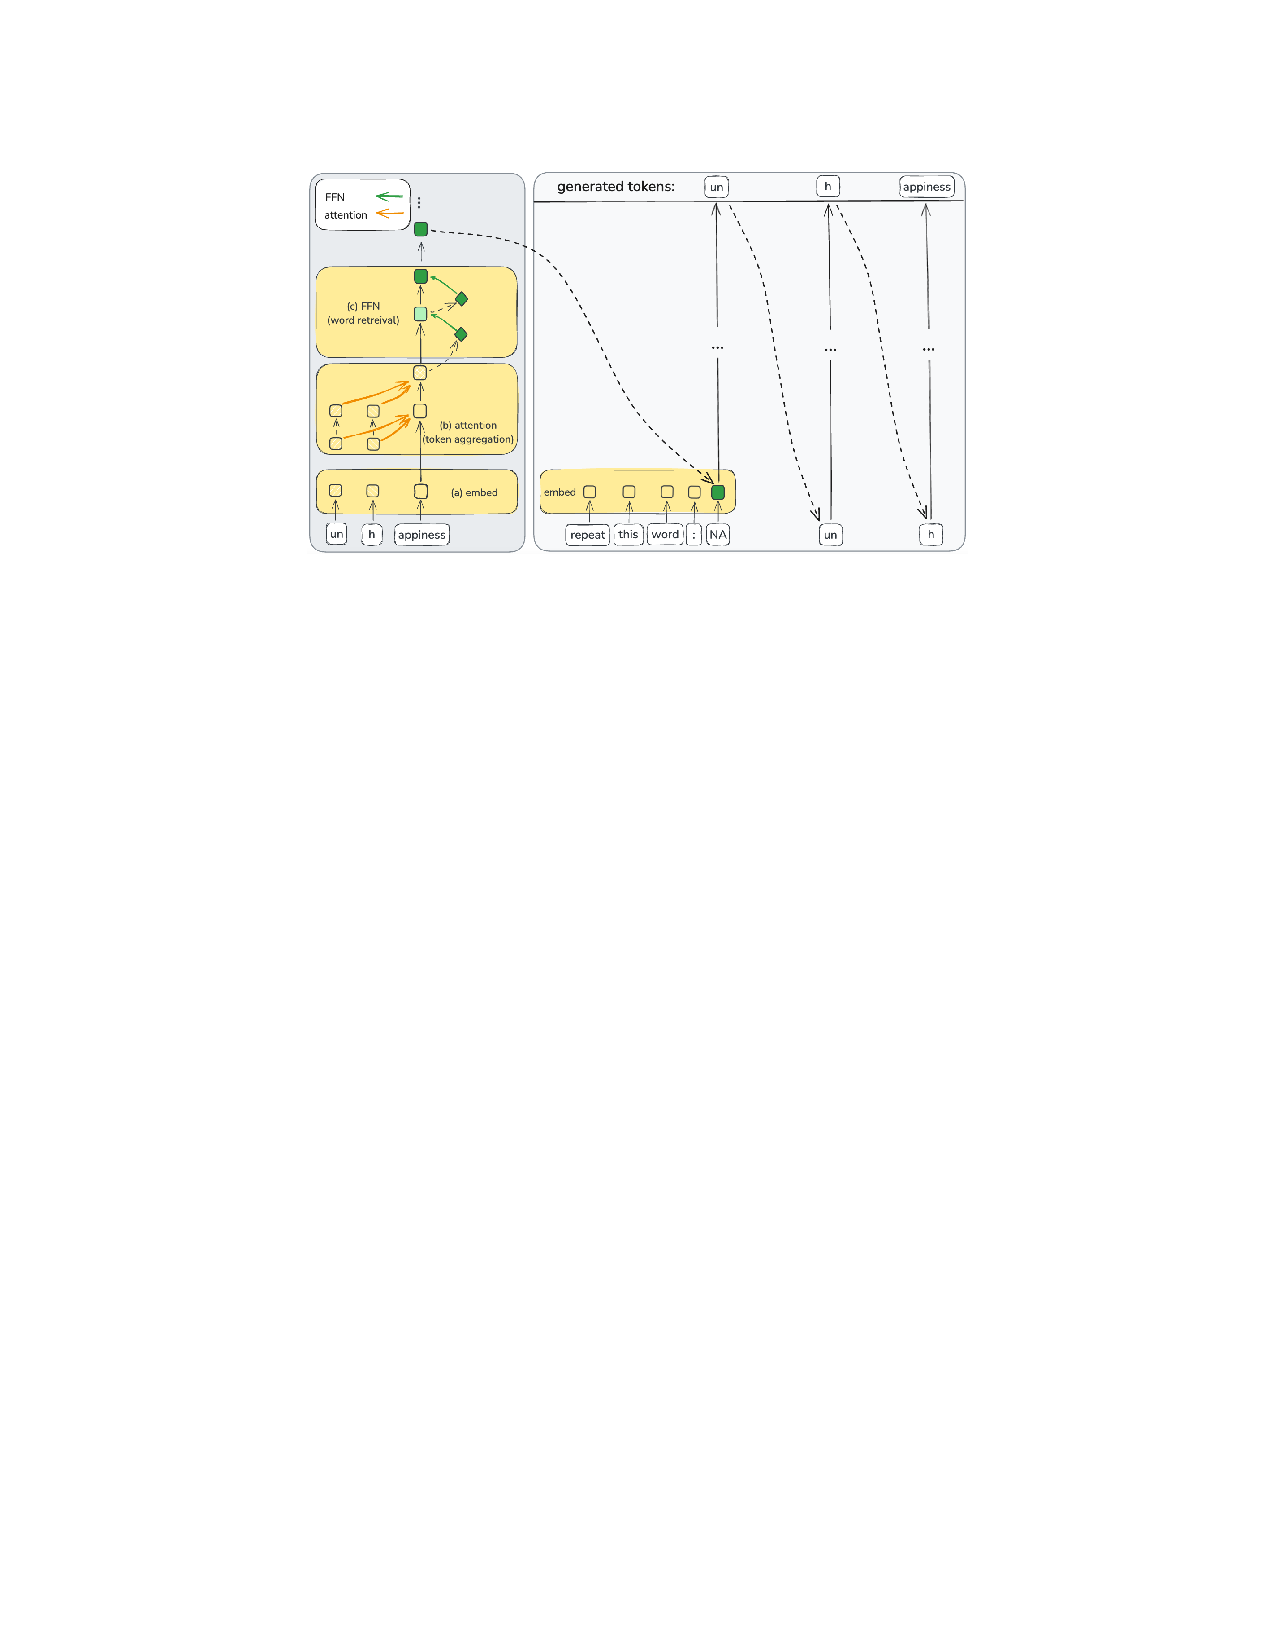
\includegraphics[width=\linewidth]{figura-1-artigo.pdf}
\end{column}
\begin{column}{0.42\textwidth}
\begin{enumerate}\setlength{\itemsep}{0.6em}
\item \textbf{Atenção:} reúne informações dos fragmentos no último token.
\item \textbf{FFNs:} redes de cada camada contribuem para reconstruir a representação da palavra.
\end{enumerate}
\small À direita, o vetor extraído é inserido em outro contexto para testar a recuperação da palavra.
\end{column}
\end{columns}
\fonte{Figura 1, reproduzida do artigo; seção 5}
\end{frame}
% 5 | 3:20--4:25 | Lucas Rapozo
\begin{frame}{Evidência 1: palavras versus não palavras}
\begin{itemize}\setlength{\itemsep}{0.65em}
\item Conjunto balanceado: 10 mil palavras em inglês e não palavras construídas por embaralhamento de tokens.
\item Um classificador k-NN tenta distinguir os grupos usando os estados internos de cada camada.
\item \textbf{Último token:} pico de \textbf{89\% de acurácia na camada 13}.
\item \textbf{Controle com o penúltimo token:} chega a 61\%, em palavras de três tokens ou mais.
\end{itemize}
\fonte{seção 3 e Figura 2; acurácia do classificador auxiliar, não do LLM em tarefas gerais}
\end{frame}
% 6 | 4:25--5:50 | Lucas Rapozo
\begin{frame}{Evidência 2: recuperar a palavra inteira}
\begin{tabularx}{\textwidth}{@{}p{3.1cm}XX@{}}
\toprule
\textbf{Experimento} & \textbf{Como verificar} & \textbf{Resultado no Llama2-7B}\\\midrule
Palavra de um token, dividida artificialmente & Comparar o estado interno com os vetores de entrada (logit lens adaptado). & 93,2\% recuperadas em pelo menos uma camada.\\[0.35em]
Palavra originalmente de vários tokens & Inserir o vetor em outro prompt e pedir repetição (Patchscopes). & 77,4\% recuperadas em pelo menos uma camada.\\\bottomrule
\end{tabularx}\par
\vspace{0.2cm}
\textbf{Limite:} 22,6\% das palavras de vários tokens não foram recuperadas por esse procedimento em nenhuma camada.
\fonte{seções 4.1 e 4.2; taxas acumuladas entre camadas, não acurácia de uma única camada}
\end{frame}
% 7 | 5:50--7:00 | Lucas Rapozo
\begin{frame}{Evidência 3: intervir nas redes FFN}
\begin{itemize}\setlength{\itemsep}{0.65em}
\item Os autores removem atualizações FFN associadas à palavra completa, em cerca de 5\% das camadas.
\item Em palavras com sufixos divididas artificialmente, a recuperação cai de \textbf{85\% para 18\%}.
\item Remover a mesma quantidade de atualizações aleatórias tem pouco ou nenhum efeito nesse teste.
\item A intervenção reforça o papel das FFNs no mecanismo, além da observação de semelhanças entre vetores.
\end{itemize}
\fonte{seção 5.1; ablação em palavras com sufixos ing, ion e est}
\end{frame}
% 8 | 7:00--7:55 | Antoniel Magalhães
\begin{frame}{Aplicação: ampliar o vocabulário}
\begin{enumerate}\setlength{\itemsep}{0.6em}
\item Extrair a representação de uma palavra de vários tokens na primeira camada em que ela é recuperada.
\item Aprender projeções para gerar suas novas entradas nas matrizes de entrada e saída.
\item Refinar as novas representações com matrizes adicionais, mantendo os demais parâmetros congelados.
\end{enumerate}
\vspace{0.15cm}
\textbf{Distinção importante:} os pesos centrais ficam fixos, mas há aprendizado de projeções e treinamento de refinamento.
\fonte{seção 6 e Figura 6; ``sem fine-tuning'' não significa ausência de treinamento auxiliar}
\end{frame}
% 9 | 7:55--9:00 | Antoniel Magalhães
\begin{frame}{Menos tokens, acurácia próxima da original}
\textbf{Expansão do vocabulário no Llama2-7B}
\begin{tabularx}{\textwidth}{@{}Xrrr@{}}
\toprule
\textbf{Conjunto} & \textbf{Original} & \textbf{Método} & \textbf{Menos tokens}\\\midrule
WikiText-103 & 52,2\% & 51,9\% & 10,5\%\\[0.4em]
PubMed & 51,7\% & 51,1\% & 13,5\%\\[0.4em]
Wiki40B em árabe & 53,5\% & 53,2\% & 14,5\%\\\bottomrule
\end{tabularx}\par
\vspace{0.2cm}
\begin{itemize}\setlength{\itemsep}{0.4em}
\item Original e Método: acurácia top-1 em nível de token, na linha geral da Tabela 1.
\item Redução medida na codificação do texto; não equivale a uma redução comprovada de igual valor na latência.
\end{itemize}
\fonte{Tabela 1 e Apêndice H, Tabela 5}
\end{frame}
% 10 | 9:00--10:00 | Antoniel Magalhães
\begin{frame}{Síntese e limites da evidência}
\begin{itemize}\setlength{\itemsep}{0.7em}
\item Os experimentos sustentam a reconstrução de palavras no último token, sobretudo em camadas iniciais e intermediárias.
\item As representações podem ampliar o vocabulário e reduzir o número de tokens processados.
\item Recuperar uma palavra não comprova compreensão semântica completa; falhar na recuperação não prova ausência de conhecimento.
\item A aplicação foi avaliada no Llama2-7B em três conjuntos. Generalização e ganhos de tempo exigem avaliações adicionais.
\end{itemize}
\fonte{seções 4--7 e Apêndice H; limites interpretativos destacados pela equipe}
\end{frame}
\appendix
\begin{frame}[noframenumbering]{Artigo de referência}
\textbf{From Tokens to Words: On the Inner Lexicon of LLMs}

Guy Kaplan; Matanel Oren; Yuval Reif; Roy Schwartz.

The Hebrew University of Jerusalem. \textit{ICLR 2025}.

\href{https://arxiv.org/abs/2410.05864v4}{arXiv:2410.05864v4}, versão de 3 de março de 2025.

\href{https://github.com/schwartz-lab-NLP/Tokens2Words}{Código: schwartz-lab-NLP/Tokens2Words}

\small Síntese baseada no PDF fornecido. A Figura 1 foi reproduzida do artigo; tabelas dos slides são recortes dos resultados, com identificação da métrica e do experimento.
\end{frame}
\end{document}
